\subsection{Task 1}
%%%%%%%%%%%%%%%%%% Grid Convergence %%%%%%%%%%%%%%%%%%%%
\subsubsection{Grid Convergence}
\noindent The geometry is modeled as an axisymmetric slice of the circular pipe using the Design Modeler tool of ANSYS Workbench. The same geometry is meshed into elements of different sizes to check whether the grid convergence is achieved or not. The element sizes tried to check convergence are as follows:

\begin{itemize}
    \item $10^{-2}$ meters
    \item $10^{-3} $ meters
    \item $5* 10^{-4}$  meters
\end{itemize}

\begin{figure}[h]
    \centering
    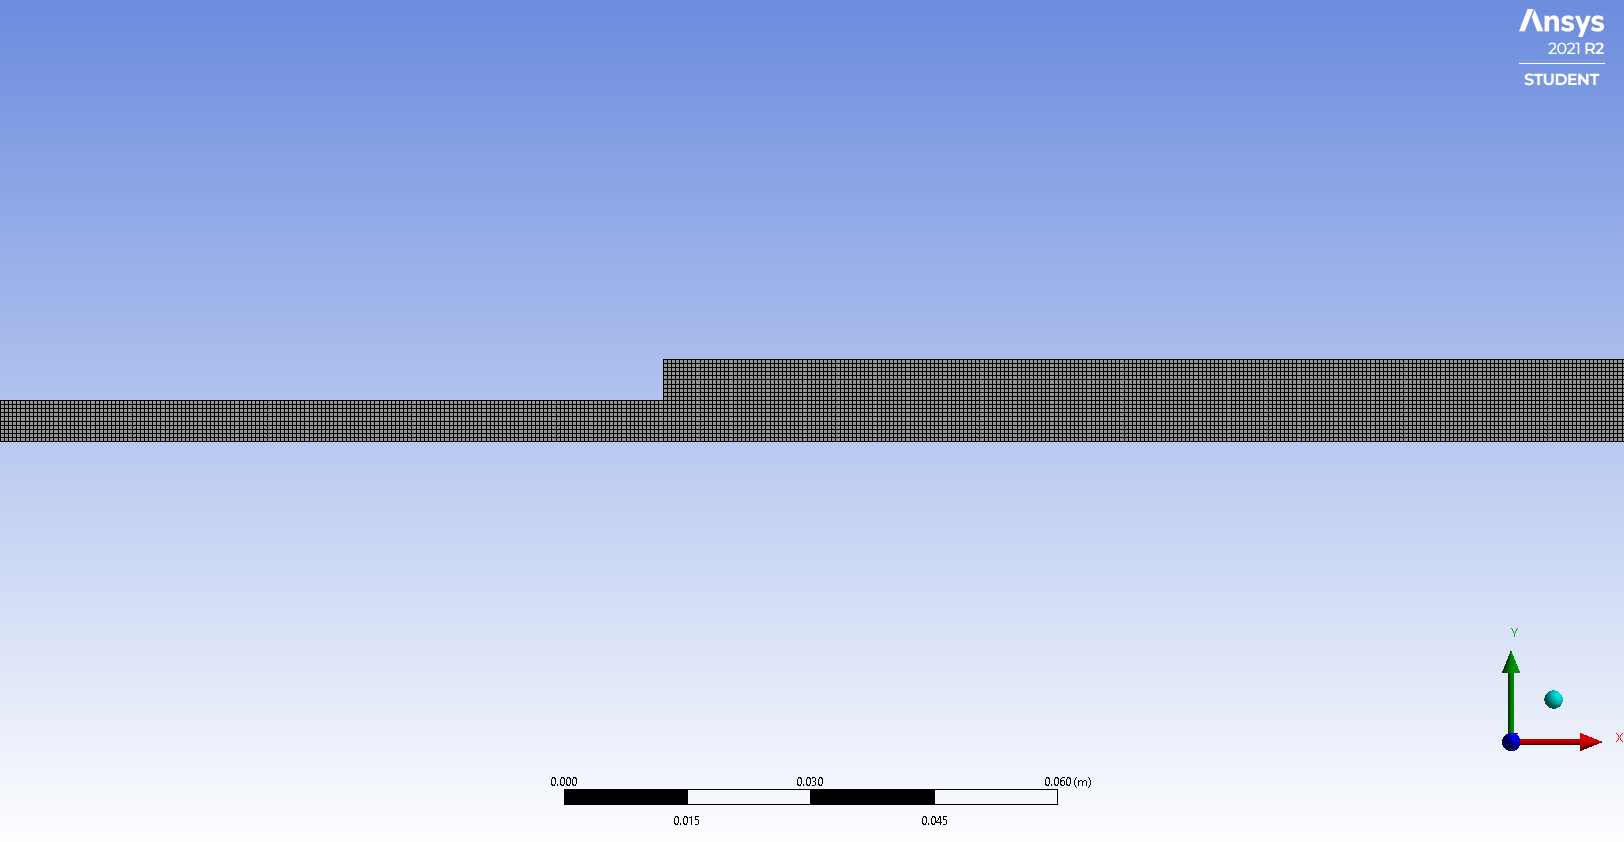
\includegraphics[width=16cm]{images/task1/5e04mesh.png}
    \caption{Mesh of the geometry with $5*10^{-4}$ meters as element size}
    \label{fig:mesh_fig}
\end{figure}


\noindent It was determined that after $5*10^{-4}$ meters of size, the results have been converged. For this condition, node and element numbers can be seen from Table \ref{table:mesh_info}, the mesh consisted of 12721 nodes and 12000 elements. While Figure \ref{fig:mesh_fig} shows the mesh from a broader perspective, Figure \ref{fig:closer_look} shows a zoomed view of the mesh created. Also, the student version of ANSYS struggled highly with smaller mesh sizes anyways.

\begin{table}[h]
\caption{Relevant Information On the Mesh}

\centering
\begin{tabular}{l|c}
\hline
\hline
Parameter          & Value                      \\ \hline
Element Size       & $5*10^{-4}m$ \\
Number of elements & 12000                      \\
Number of nodes    & 12721   

\end{tabular}

\label{table:mesh_info}
\end{table}


\begin{figure}[h]
    \centering{
    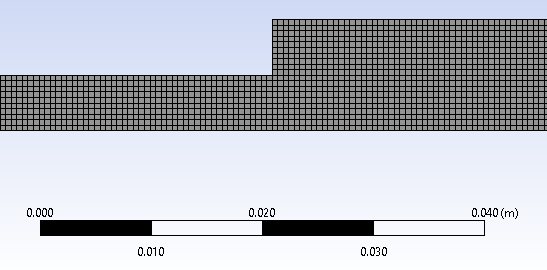
\includegraphics[width = 11cm]{images/task1/closer_look.png}
    \caption{A closer view of the mesh.}
    \label{fig:closer_look}}
\end{figure}


\noindent In order to conclude that the results have been converged, velocity profiles of the fluid at different cross-sections have been compared until little to no improvement on the results have been observed on results. As can be seen from Figure \ref{fig:convergence}, the results are almost the same between the element sizes of a and b. This relation is also closely observed on the velocity profiles from selected cross sections of the pipe.\\

\begin{figure}[H]

    \centering{
    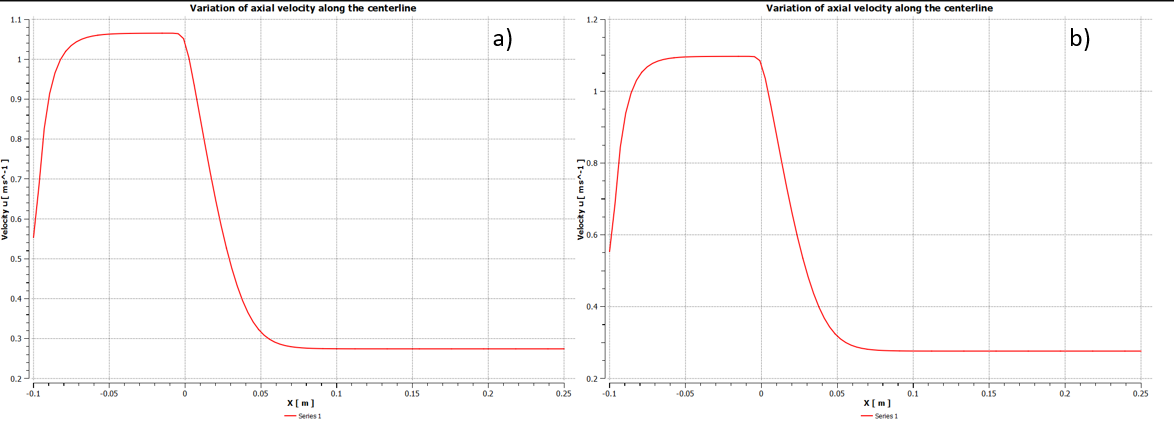
\includegraphics[width=16cm]{images/task1/convergence.png}
    \caption{Axial velocities along the centerline: a) Element size $10^{-3}$meters, b) Element size $5*10^{-4}$ meters.}
    \label{fig:convergence}}
\end{figure}

\noindent Figure \ref{fig:convergence2} shows the similarity between two different mesh sizes that have been tried and checked for grid convergence. The velocity profiles are taken from x=1cm for both cases. While Figure-\ref{fig:convergence2}.a is smoother, the results are almost exactly the same for both cases.

\begin{figure}[H]
    \centering{
    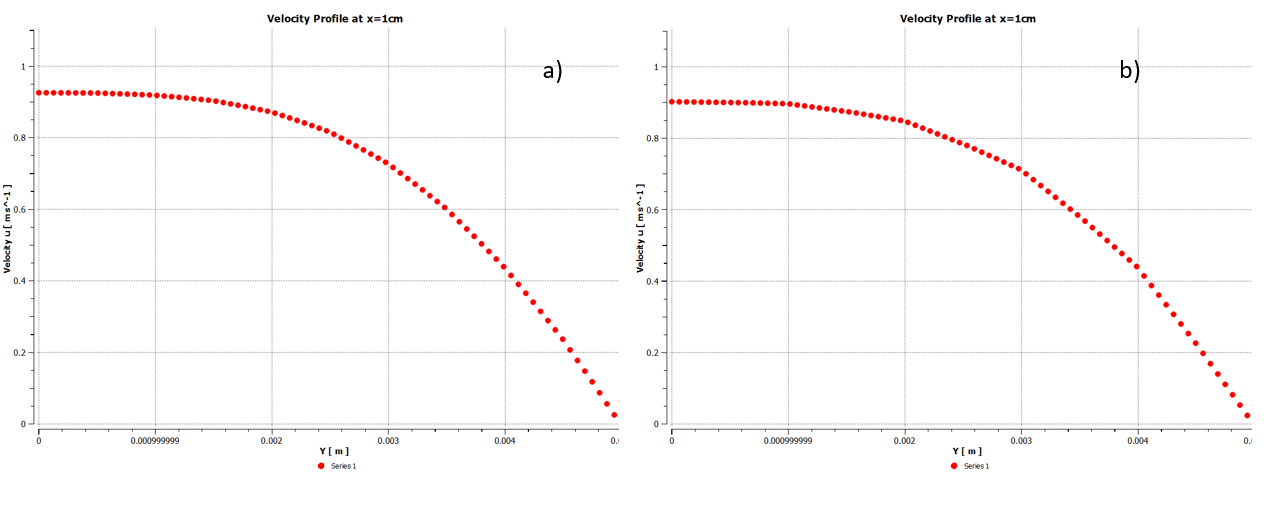
\includegraphics[width=14cm]{images/task1/convergence2.png}
    \caption{Comparison of the velocity profiles of element sizes at x=1cm shown on Figure \ref{fig:convergence}.}
    \label{fig:convergence2}}
\end{figure}


\noindent As requested from the project prompts, those 3 different mesh sizes are further compared by
plotting the axial velocity profiles at the axial locations of x = 0.5 cm, 1 cm,
1.5 cm, 2 cm, and 3 cm. Those plots can be seen from Figure \ref{fig:axials}. When compared, of course due to the difference in number of elements, finer mesh produces a smoother curve as expected since it contains more data points. However, the values kept at the same point are the same and the values are not changing with decreasing element size or increasing node count.


\begin{figure}[H]
    \centering
    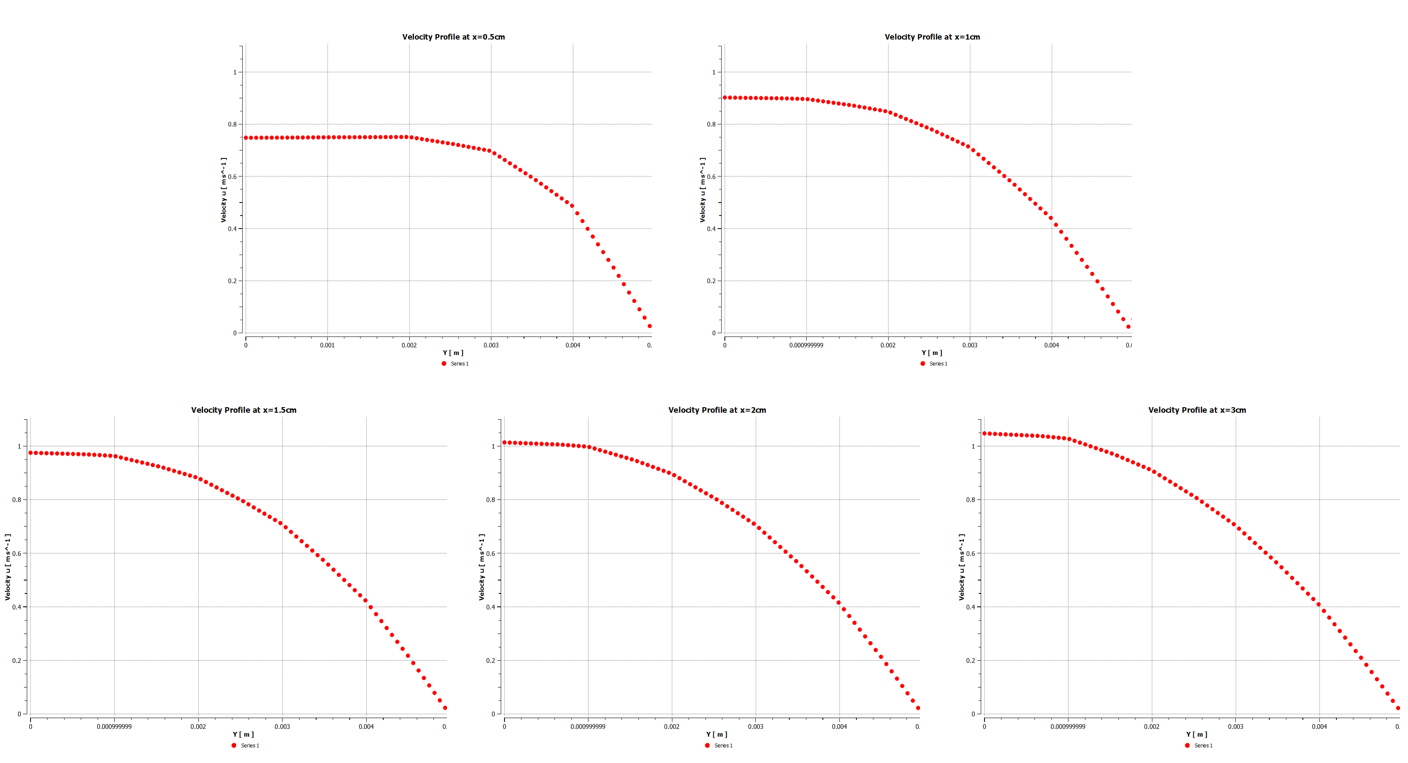
\includegraphics[width=15cm]{images/task1/e_03_total.png}
    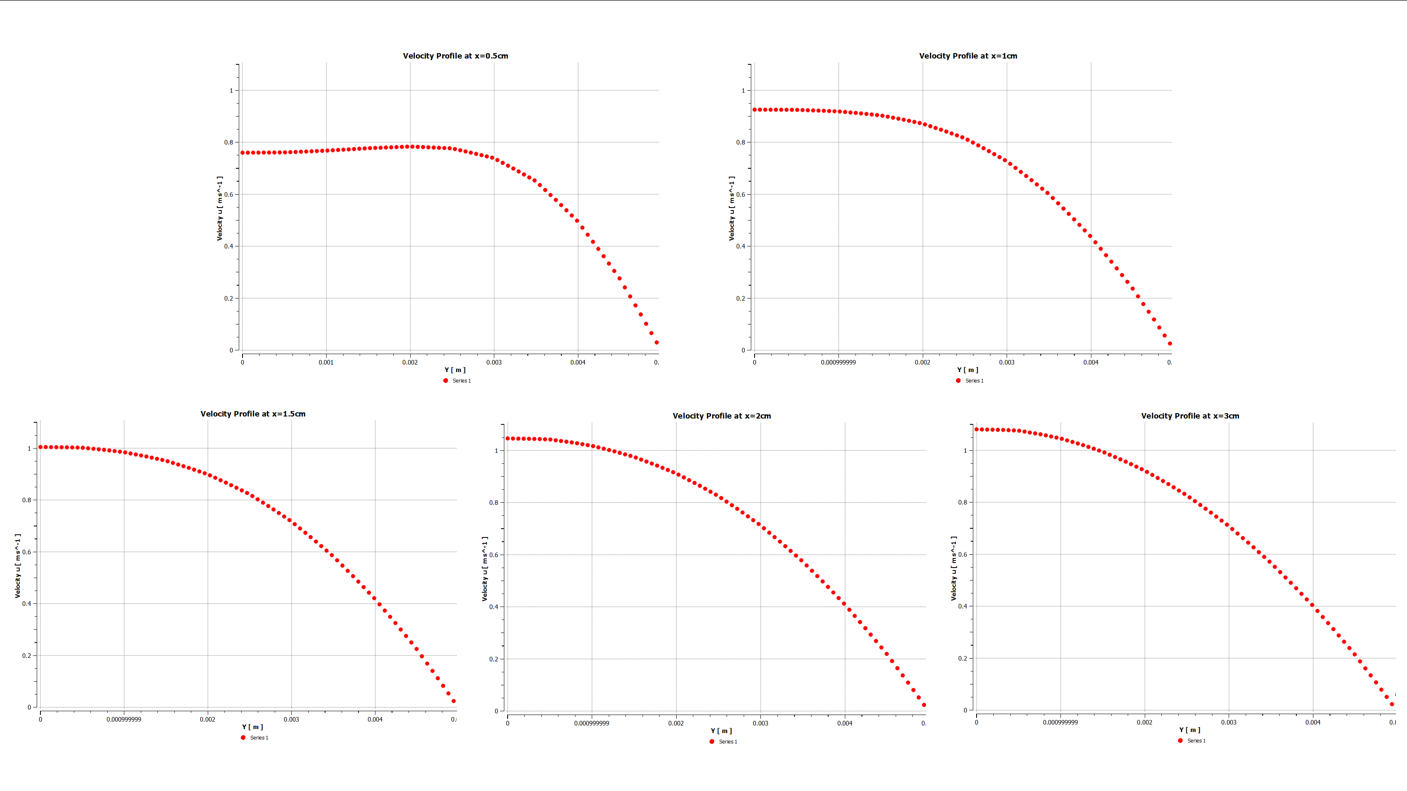
\includegraphics[width=15cm]{images/task1/5e_04_total.png}
    \caption{Velocity Profiles at x = 0.5, 1, 1.5, 2 and 3cm for element sizes $10^{-3}$m (above 5), and $5*10^{-4}$m (lower 5).}
    \label{fig:axials}
\end{figure}



%%%%%%%%%%%%%%% Residuals and Calculations %%%%%%%%%%%%
\subsubsection{Residuals and Calculations}
Once the calculation is run, we must be sure that a steady state condition is achieved. The reason for this check is due to nature of our solver and numerical methods used. Our solver stops the calculations on one of these two conditions:

\begin{itemize}
    \item Residual error in each step have dropped under a set threshold determined by the user and the solution is converged.
    \item Maximum number of steps have achieved.
\end{itemize}

\noindent A plot of the residuals have been drawn and can be seen on Figure \ref{fig:residuals}. As can be seen, 
all of the tracked values have gone under $10^{-6}$ which is low enough to state that a steady state has been achieved at the step.

\begin{figure}[H]
    \centering
    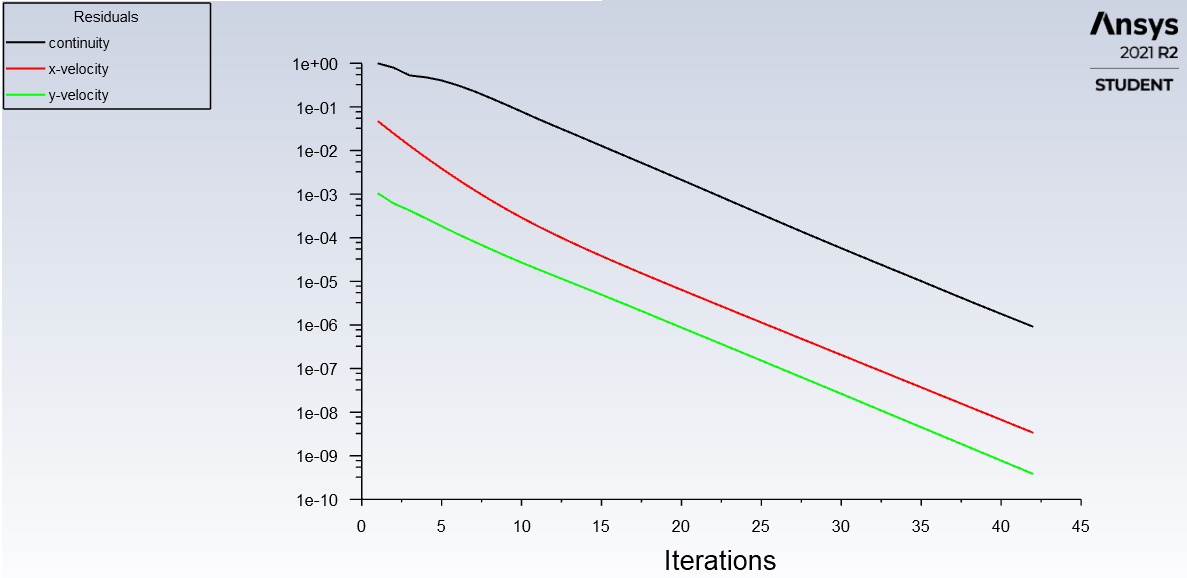
\includegraphics[width=15cm]{images/task1/residuals.png}
    \caption{Plot of the Residuals for Task 1}
    \label{fig:residuals}
\end{figure}
\\
\\
\noindent Velocity profiles at several cross sections along the centerline can be seen on Figure \ref{fig:velprof3}. This plot can be validated by using the \textbf{Poiseuille-Hagen} solution by using the formula given below. 

\begin{equation}
    u = 2V_{avg} * (1- \frac{r^{2}}{R^{2}})
    \label{eq:hagen}
\end{equation}
\\
\\
\noindent Where $V_{avg}$ is the average velocity of the fluid inside the pipe, $R$ is the radius of the pipe 
and the $r$ is the radial distance of the point from the centerline.

\begin{figure}[H]
    \centering
    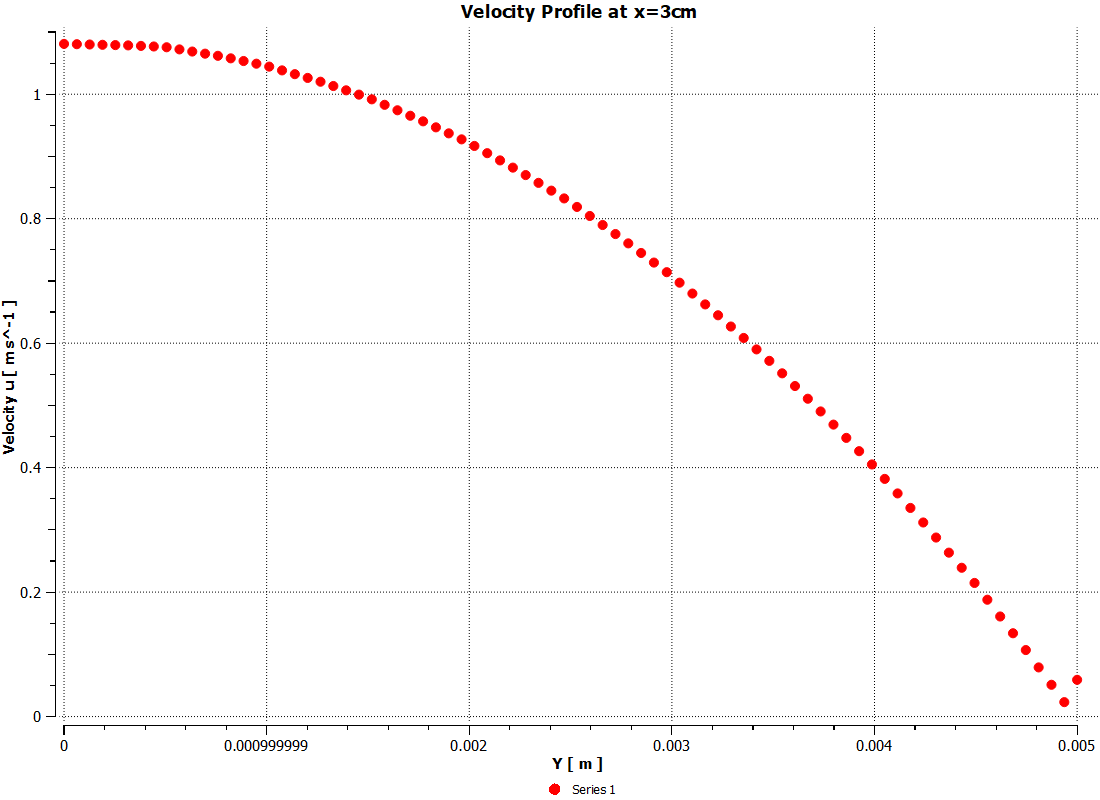
\includegraphics[width=14cm]{images/task1/vel_prof_3.png}
    \caption{Velocity Profile at x=3cm}
    \label{fig:velprof3}
\end{figure}

\noindent While not perfect, it can be clearly said that our simulation solution agrees with the given theoretical equations used to model these flows. When we plug in the values to equation \ref{eq:hagen}, we obtain the following solution:

\[ 2*0.554m/s * \Big(1 - \frac{0}{0.1^{2}m^{2}}\Big) = 1.108 m/s \] 

\noindent when evaluated at the centerline. This value is \textbf{within $1\%$} of the value we obtained from the simulation. A similar picture is seen when looked at the axial velocity profiles along the centerline of the pipe. A plot can be seen from Figure \ref{fig:axial}, the values are again in agreement with the theoretical values and become closer as the boundary layer is formed throughout the length of the pipe. 

\begin{figure}[H]
    \centering
    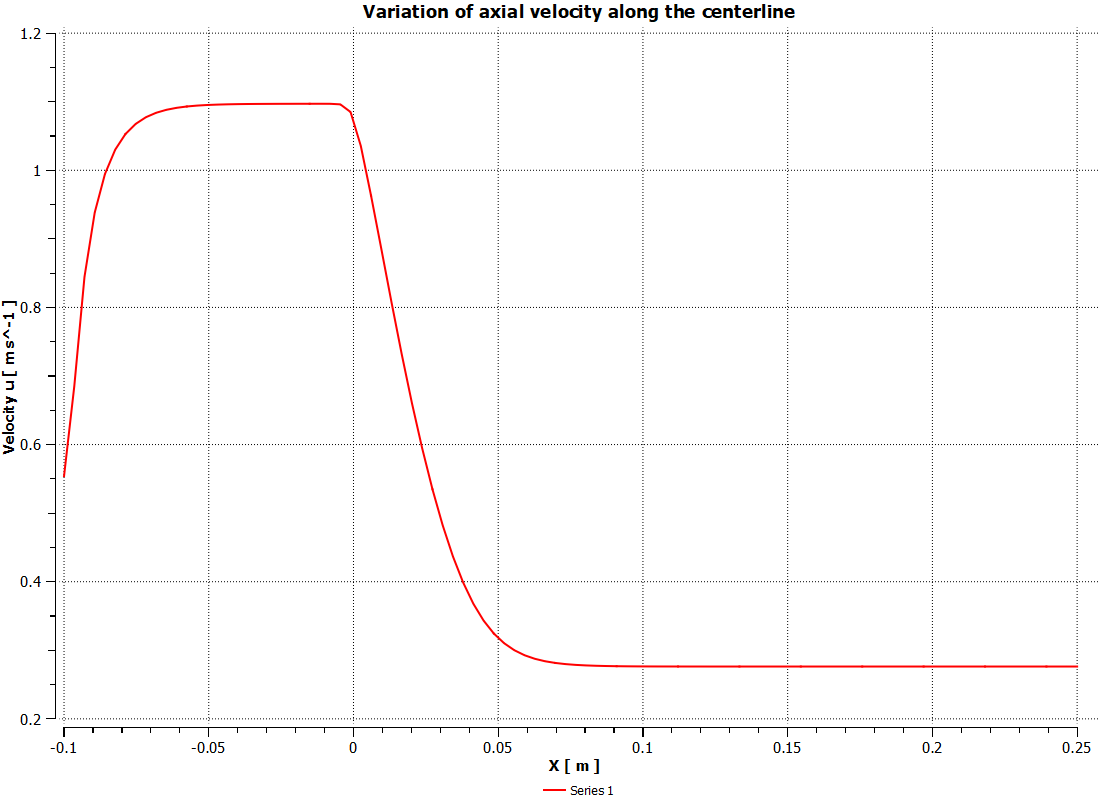
\includegraphics[width=15cm]{images/task1/axial.png}
    \caption{Axial velocities along the centerline}
    \label{fig:axial}
\end{figure}

\noindent To further show the validation of the results, velocity profiles at $x=5$ and $x=7.5$cm have been plotted which can be seen from Figure \ref{fig:vel_profiles_hagen}. Also, using MATLAB, velocity profile at x=5cm have been plotted with the Hagen equation on the same plot to show how close the data are to each other on Figure \ref{fig:matlab_hagen}.




\begin{figure}[H]
 \centering
\begin{subfigure}{.5\textwidth}
  \centering
  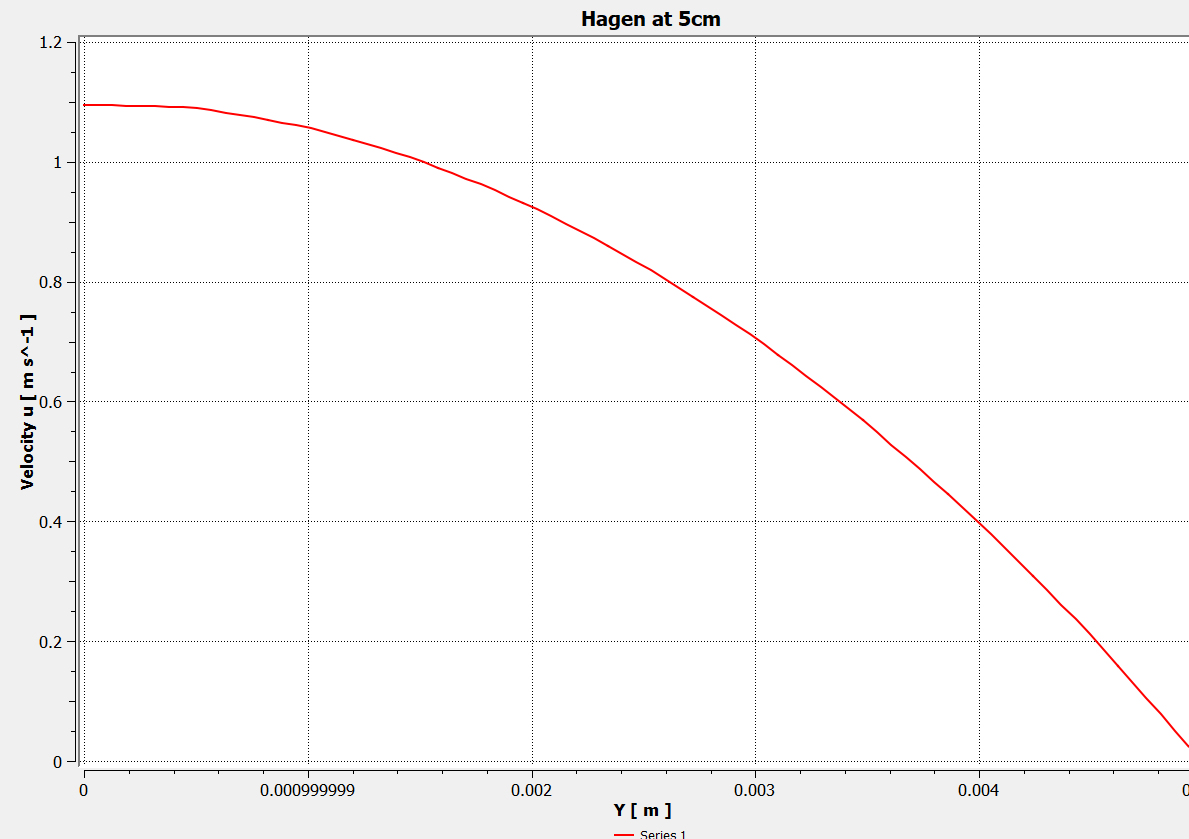
\includegraphics[width=.9\linewidth]{images/task1/hagen5.png}
  \caption{Velocity Profile at x=5cm}
  \label{fig:velprof5cm}
\end{subfigure}%
~
\begin{subfigure}{.5\textwidth}
  \centering
  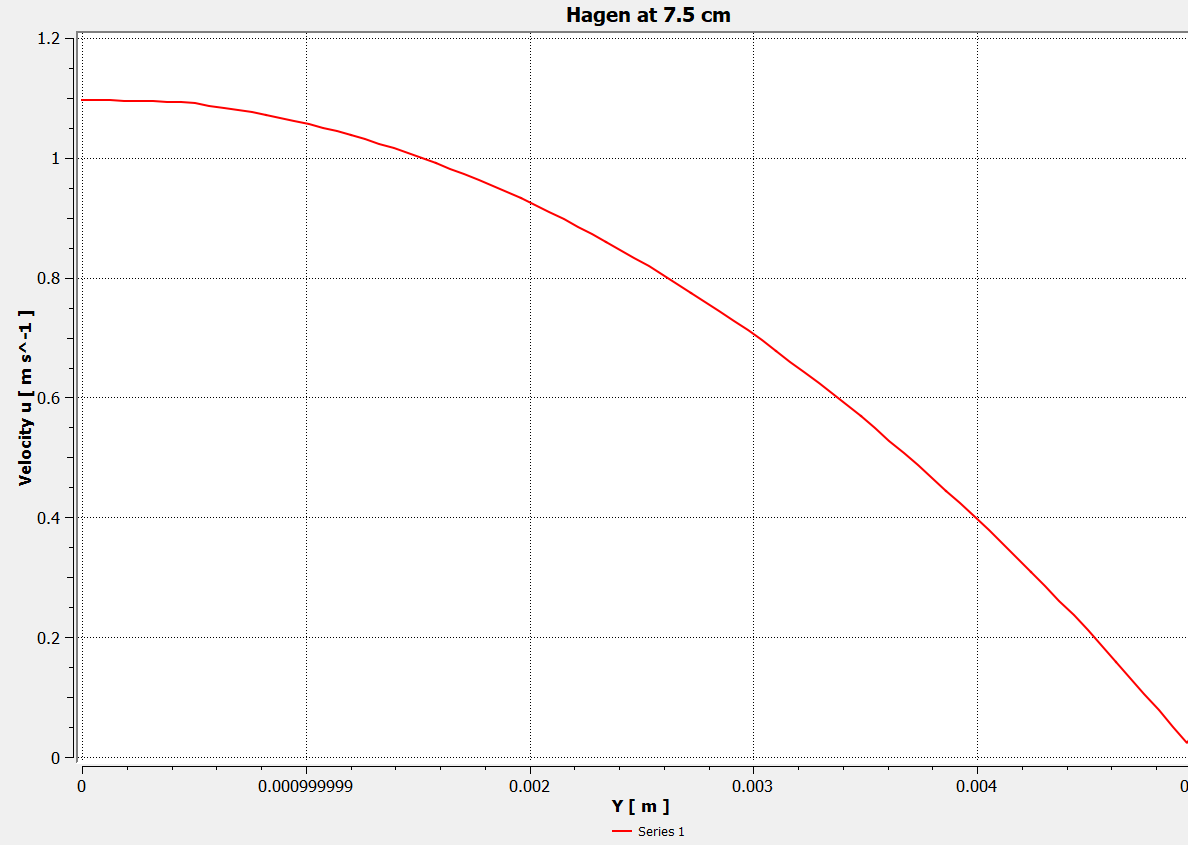
\includegraphics[width=.9\linewidth]{images/task1/hagen75.png}
  \caption{Velocity Profile at x=7.5cm}
  \label{fig:velprof75cm}
\end{subfigure}
~
\begin{subfigure}{.45\textwidth}
  \centering
  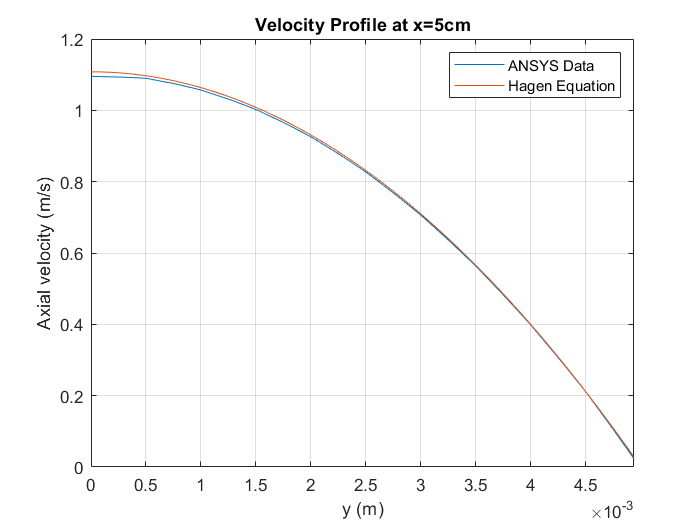
\includegraphics[width=.9\linewidth]{images/task1/hagen_ansys.png}
  \caption{My velocity profile vs the Poiseuille-Hagen equation at x=5cm}
  \label{fig:matlab_hagen}
\end{subfigure}
~
\begin{subfigure}{.45\textwidth}
  \centering
  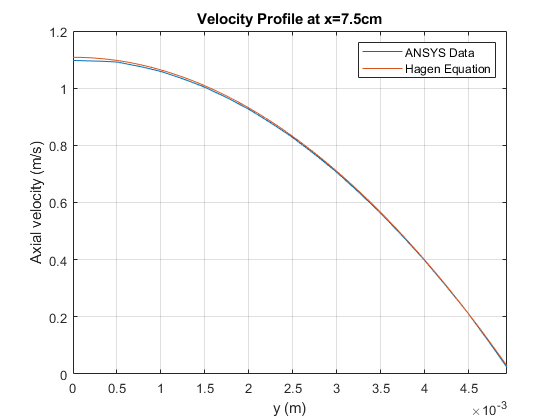
\includegraphics[width=.9\linewidth]{images/task1/hagen75_1.png}
  \caption{My velocity profile vs the Poiseuille-Hagen equation at x=7.5cm}
  \label{fig:matlab_hagen2}
\end{subfigure}
\caption{Velocity profiles and analytical comparisons}
\label{fig:vel_profiles_hagen}
\end{figure}

%%%%%%%%%%%%%%% Contours and Streamlines %%%%%%%%%%%%
\subsubsection{Contours and Streamlines}
Another useful way of interpreting the results is by visualising the obtained data into different kinds of contours and using streamlines that represent the flow inside the pipe. Using the post-processing tools of ANSYS, I have plotted the pressure contour and streamlines both separately and on top of each other. Which can be seen on Figures \ref{fig:stream} and \ref{fig:stream_w_pressure}.

\begin{figure}[H]
    \centering
    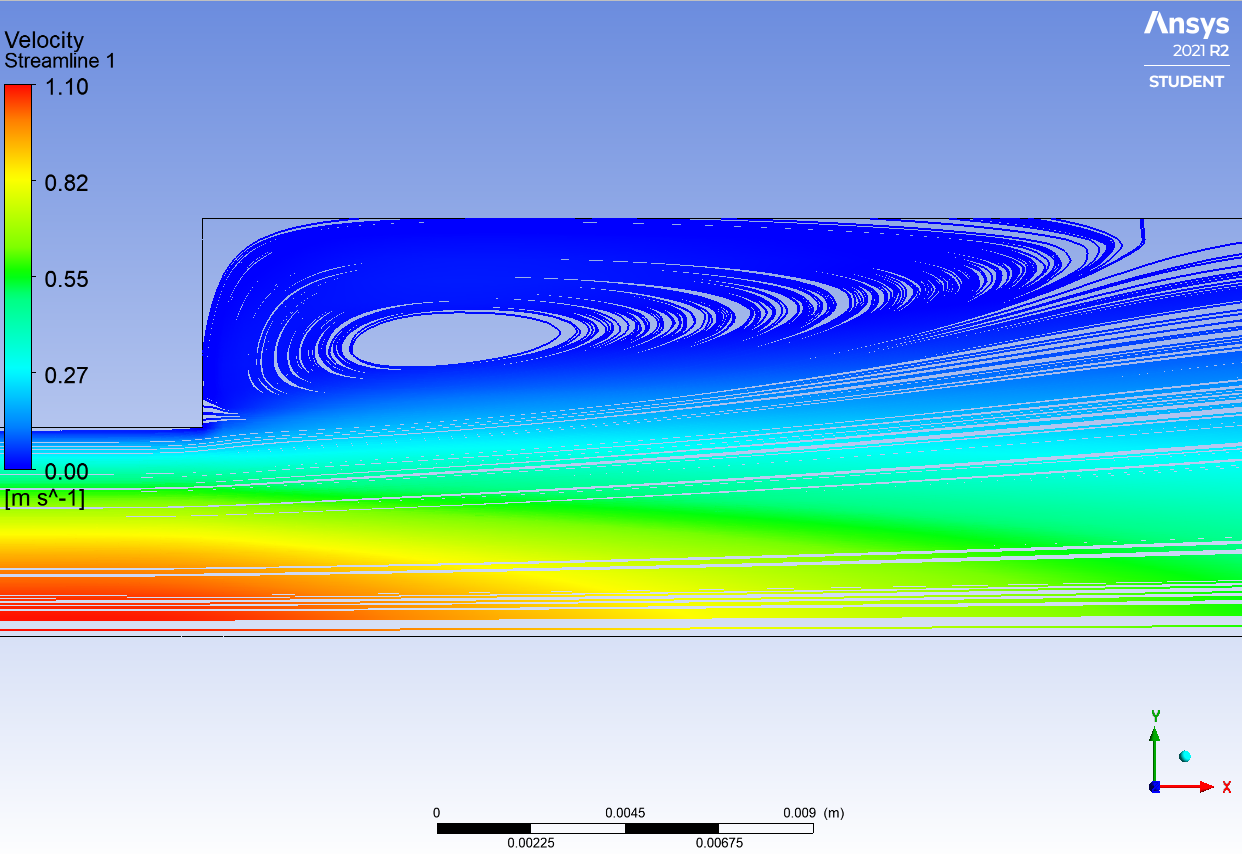
\includegraphics[width=0.9\textwidth]{images/task1/streamlines.png}
    \caption{Streamlines for the flow}
    \label{fig:stream}
\end{figure}

\begin{figure}[H]
    \centering
    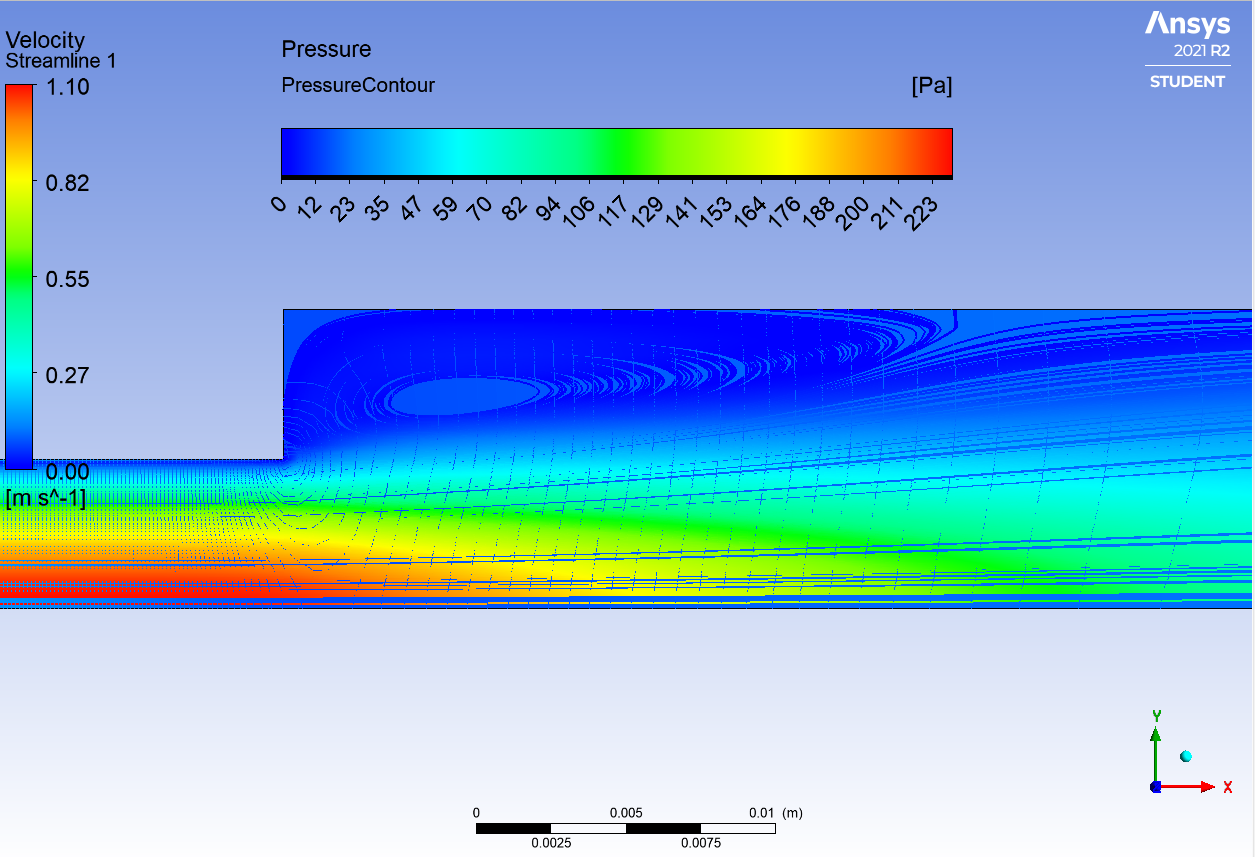
\includegraphics[width=0.9\textwidth]{images/task1/streamline_w_pressure.png}
    \caption{Streamlines for the flow plotted with pressure contours}
    \label{fig:stream_w_pressure}
\end{figure}

\noindent The streamlines for the recirculation zone can be clearly seen from the figures. This recirculation is induced by the expansion of the pipe. As the expansion causes a reduction on the pressure of the pressure at shown places, fluid particles at that point start to recirculate. \\

\noindent As expected, velocity is maximum in the centerline of the smaller pipe and pressure starts higher with the flow and dropping especially after the expansion. This drop in pressure is caused by the turbulent mixing of the flow where the pipe expands, which causes a decrease in mechanical energy.


%%%%%%%%%%%%%%% Experimental Comparison %%%%%%%%%%%%
\subsubsection{Experimental Comparison}
Now that we have made some comparisons of our results with theoretical models and equations. It is the next step to validate our results by comparing them with data obtained from previous experimental studies. To achieve this, we will be using an article published by Hammad et al.\cite{hammad_ötügen_arik_1999}. In their study, they also observed and analized the flow of a fluid through an expanding pipe.

\begin{figure}[H]
 \centering
\begin{subfigure}{.7\textwidth}
  \centering
  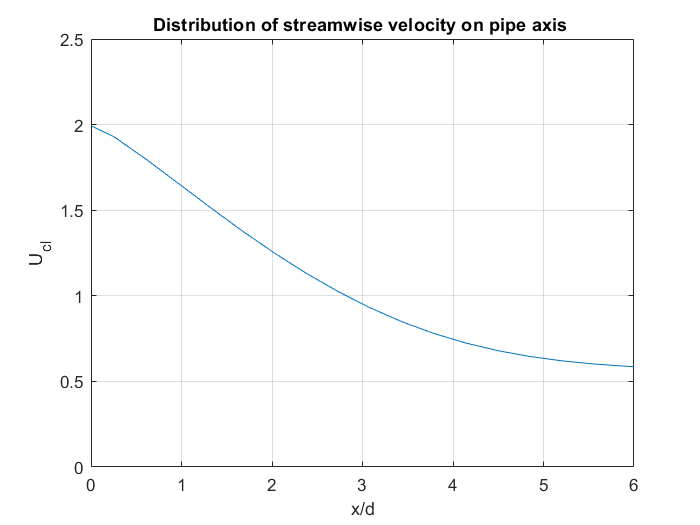
\includegraphics[width=.7\linewidth]{images/task1/x_d_norm.png}
  \caption{Distribution of streamwise velocity on pipe axis of ANSYS data.}
  \label{fig:x_d_norm}
\end{subfigure}%

\begin{subfigure}{.8\textwidth}
  \centering
  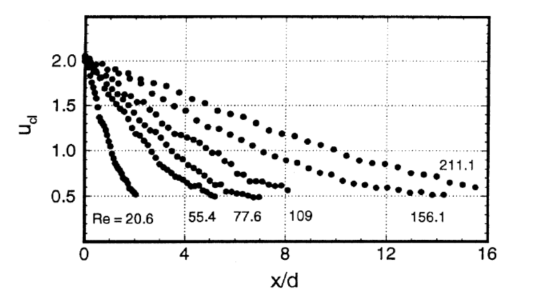
\includegraphics[width=.9\linewidth]{images/task1/x_d_norm_actual.png}
  \caption{Distribution of streamwise velocity on pipe axis from Hammad et al.\cite{hammad_ötügen_arik_1999}}
  \label{fig:x_d_norm_actual}
\end{subfigure}

\caption{Streamwise Velocity Comparison}
\label{fig:xd_norm}
\end{figure}

\noindent Figure \ref{fig:xd_norm} shows the similarities with data from our simulation and the data provided by \cite{hammad_ötügen_arik_1999}. While their chart contains data points from 6 different flows with different Reynolds numbers, the one which $Re = 55.4$ corresponds to our MATLAB plot that is shown above with very little error. This distribution makes sense since the fluid enters the second pipe with the highest velocity that is obtained from the equation \ref{eq:hagen} and that value corresponds to twice of the average velocity of the fluid. However, as the fluid moves deeper into the second pipe, the velocity at the centerline drops to around half of the average velocity.\\


\noindent Moreover, Hammad et al. provides velocity vectors for the case of $Re = 55.4$ throughout the length of the wider pipe. Once we obtain the velocity vector plots from ANSYS Fluent ourselves, a comparison can be made between our simulated data and their experimental data. 

\begin{figure}[H]
 \centering
\begin{subfigure}{.8\textwidth}
  \centering
  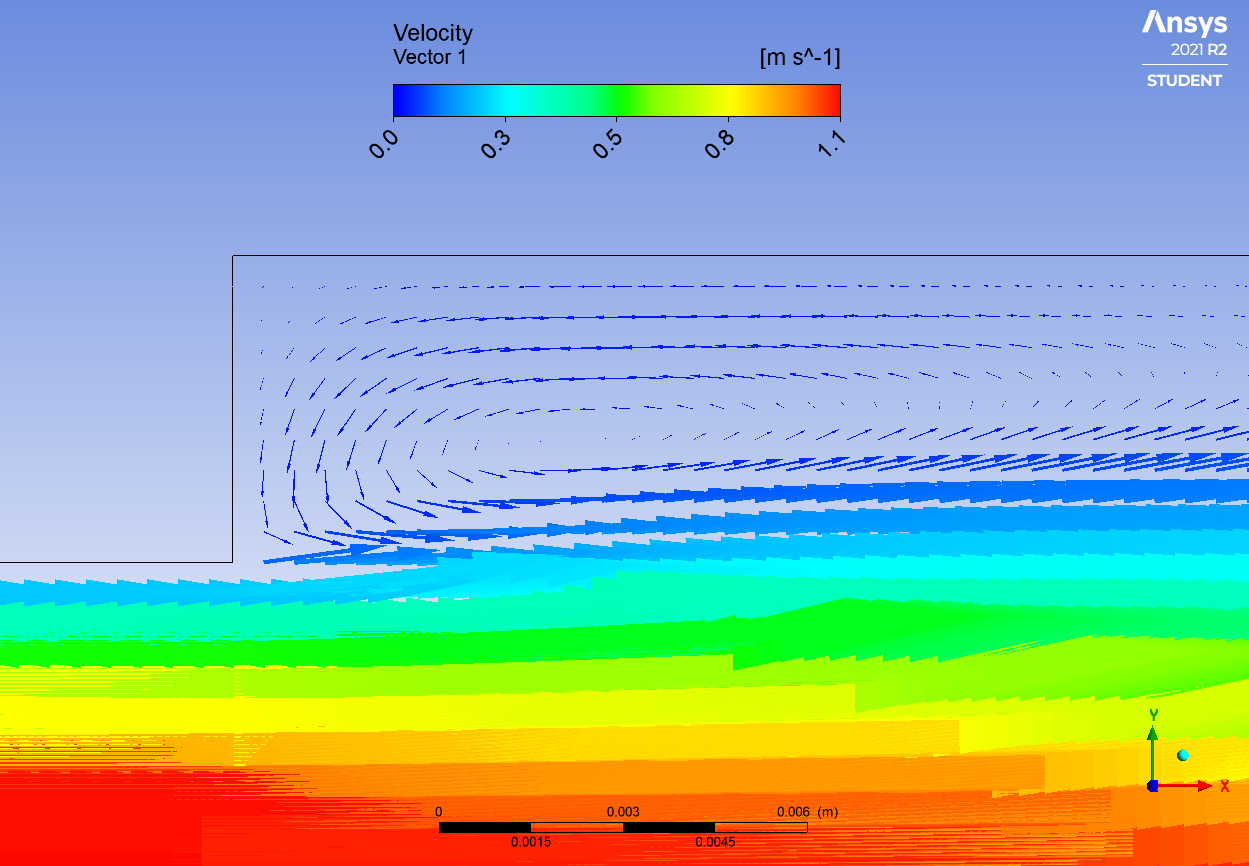
\includegraphics[width=.8\linewidth]{images/task1/vectors.png}
  \caption{Upscaled velocity vectors at the expansion.}
  \label{fig:vel_vel1}
\end{subfigure}%
\hfill
\begin{subfigure}{.8\textwidth}
  \centering
  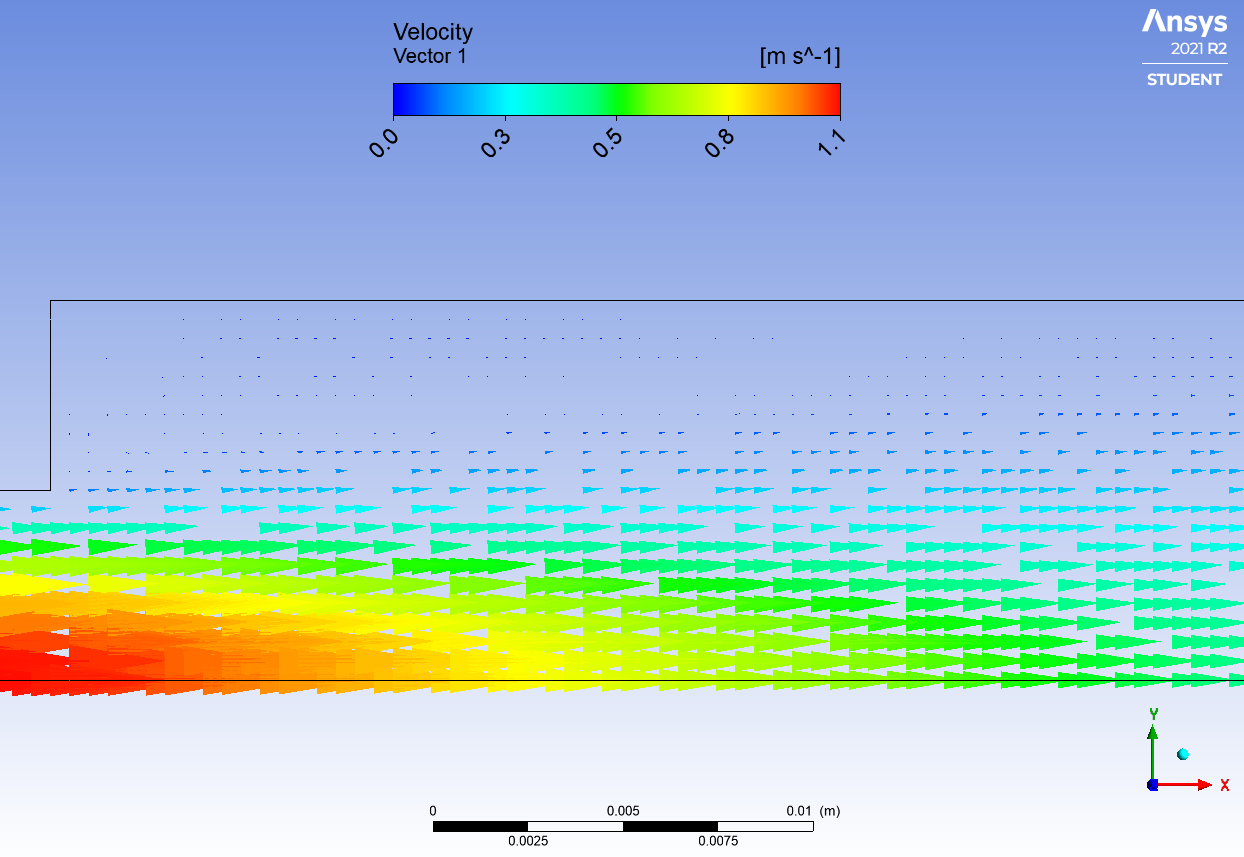
\includegraphics[width=.8\linewidth]{images/task1/vectorsplot.png}
  \caption{Velocity vectors at the expansion.}
  \label{fig:vel_vel2}
\end{subfigure}
\hfill
\begin{subfigure}{.8\textwidth}
  \centering
  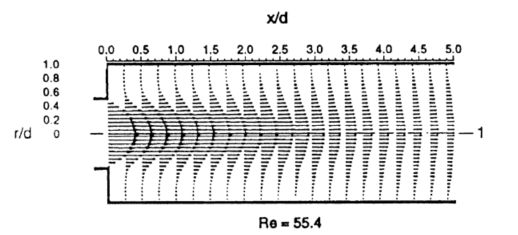
\includegraphics[width=.9\linewidth]{images/task1/vel_vectors.png}
  \caption{Measured velocity vectors from Hammad et al.\cite{hammad_ötügen_arik_1999}}
  \label{fig:vel_vel_measured}
\end{subfigure}

\caption{Streamwise Velocity Comparison}
\label{fig:vel_vec_comp}
\end{figure}

\vspace{0.5cm}
\noindent As can be seen from Figure \ref{fig:vel_vec_comp}, the measured values from the study and our Fluent simulation are in agreement. They both have maximum magnitude at the centerline and the magnitude gets smaller as the position of the vector gets farther away from the centerline. Also, as $x/d$ increases, magnitude of the vectors on the centerline decreases for both cases.
\\

\noindent Another aspect that was observed and modeled by Hammad et al. is the reattachment length of around the recirculation zone. In our case, the reattachment length is found looking at the streamlines and finding the point at which a streamline connects to the wall. The part before the reattachment point is called the recirculation zone. For this experiment, reattachment points have been found and plotted for 4 different $Re$ values. The change in the $Re$ values are made possible by changing the inlet velocities. Tested $Re$ values are 30, 55.4, 100 and 150.\\



\noindent The determination of the locations of the reattachment points is shown in Figure \ref{fig:reattach}. For all different cases, finding the reattachment point required tinkering with the number of streamlines to be drawn since in some cases. This was due to the fact that the location of the reattachment point was dependent on the concentration of the streamlines. The crosshairs and highlighted points on Figure \ref{fig:reattach}, depict the decided positions of reattachment points.


\begin{table}[H]
\caption{Reattachment lengths for Reynolds numbers}
\centering
\begin{tabular}{c|c}
\hline
Reynolds Number & Reattachment Length (m) \\ \hline
30              & 0.0141                  \\
55.4            & 0.0236                  \\
100             & 0.0430                  \\
150             & 0.0681                 
\end{tabular}
\end{table}

\noindent These numbers do follow the trendline that Hammad et al. has shown in their study and this can be shown by plotting our points over their chart, which can be seen from Figure \ref{fig:reattach_plot}. In this plot, our data points are shown with green circles. 

\begin{figure}[H]
    \centering
    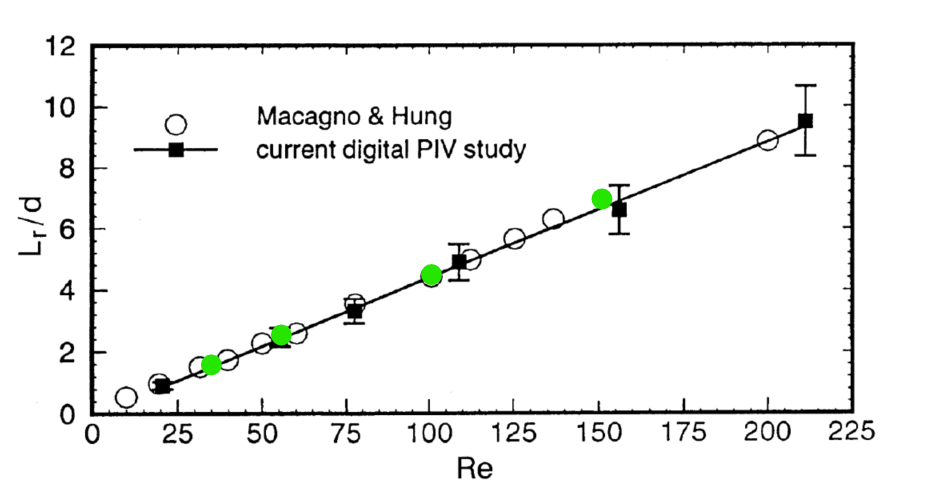
\includegraphics[width=14cm]{images/task1/reattach_plot.png}
    \caption{Plot of simulated reattachment lengths over the model of Hammad et al.}
    \label{fig:reattach_plot}
\end{figure}



\begin{figure}[H]
 \centering
\begin{subfigure}{.5\textwidth}
  \centering
  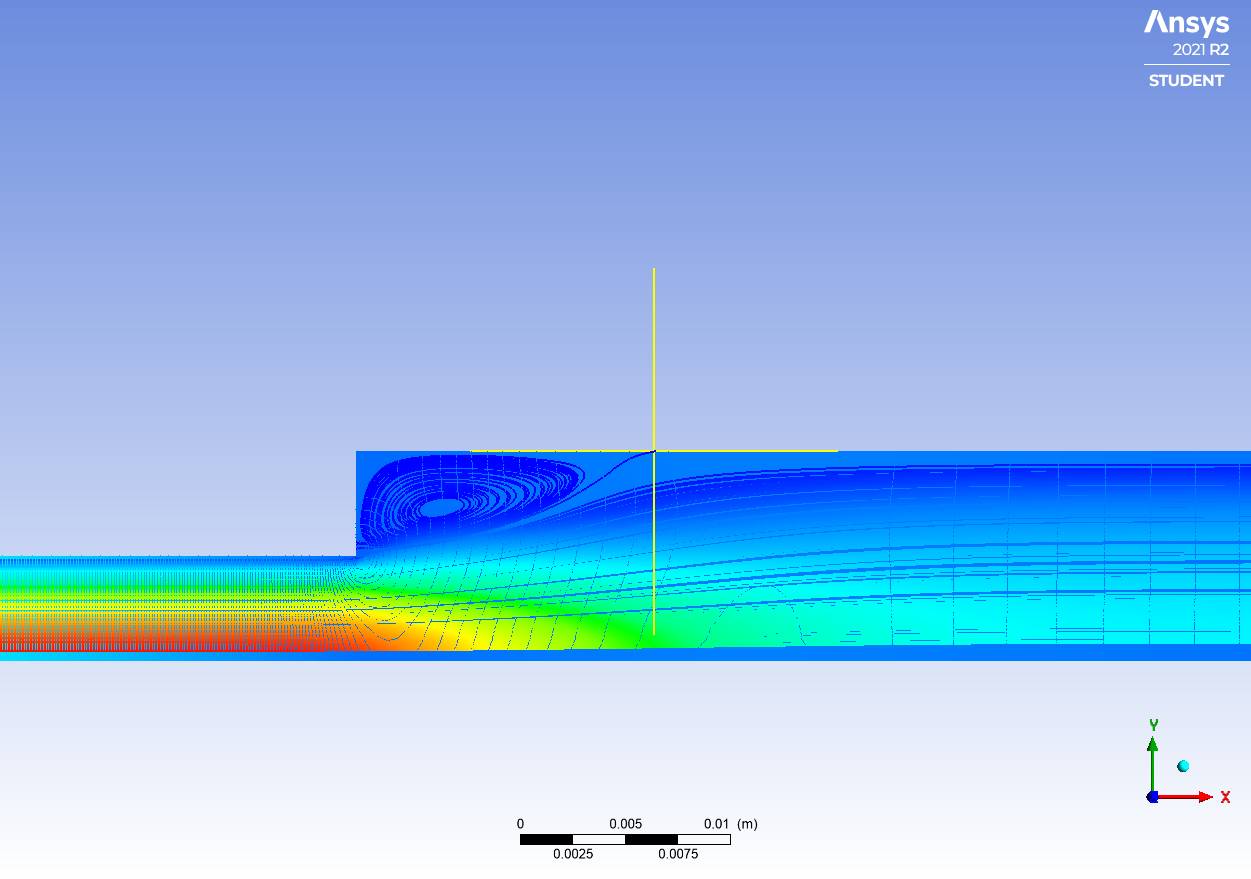
\includegraphics[width=.95\linewidth]{images/task1/030_attachement_0_0141.png}
  \subcaption{}
  \label{fig:reat_a}
\end{subfigure}%
\hfill
\begin{subfigure}{.5\textwidth}
  \centering
  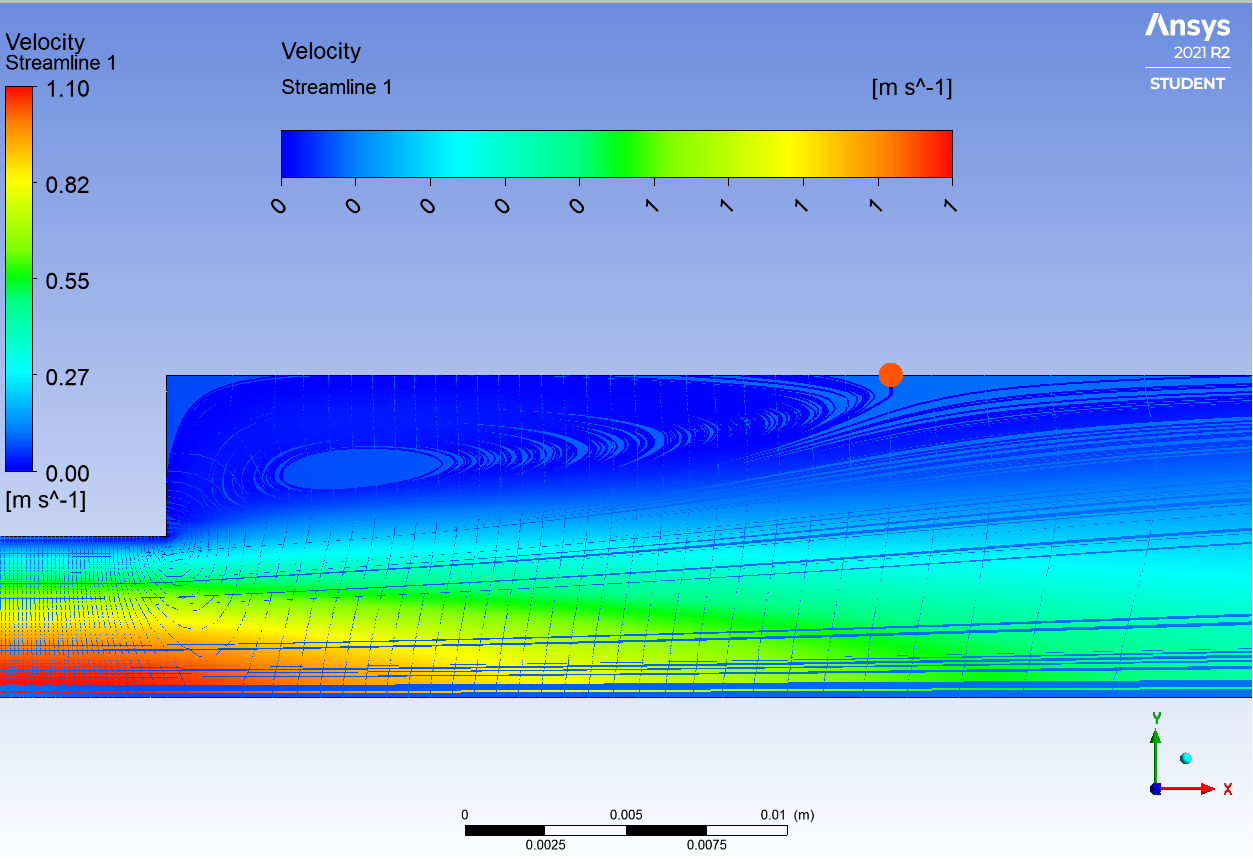
\includegraphics[width=.95\linewidth]{images/task1/0554_attachement_0_0236.png}
  \subcaption{}
  \label{fig:reat_b}
\end{subfigure}
\hfill
\begin{subfigure}{.75\textwidth}
  \centering
  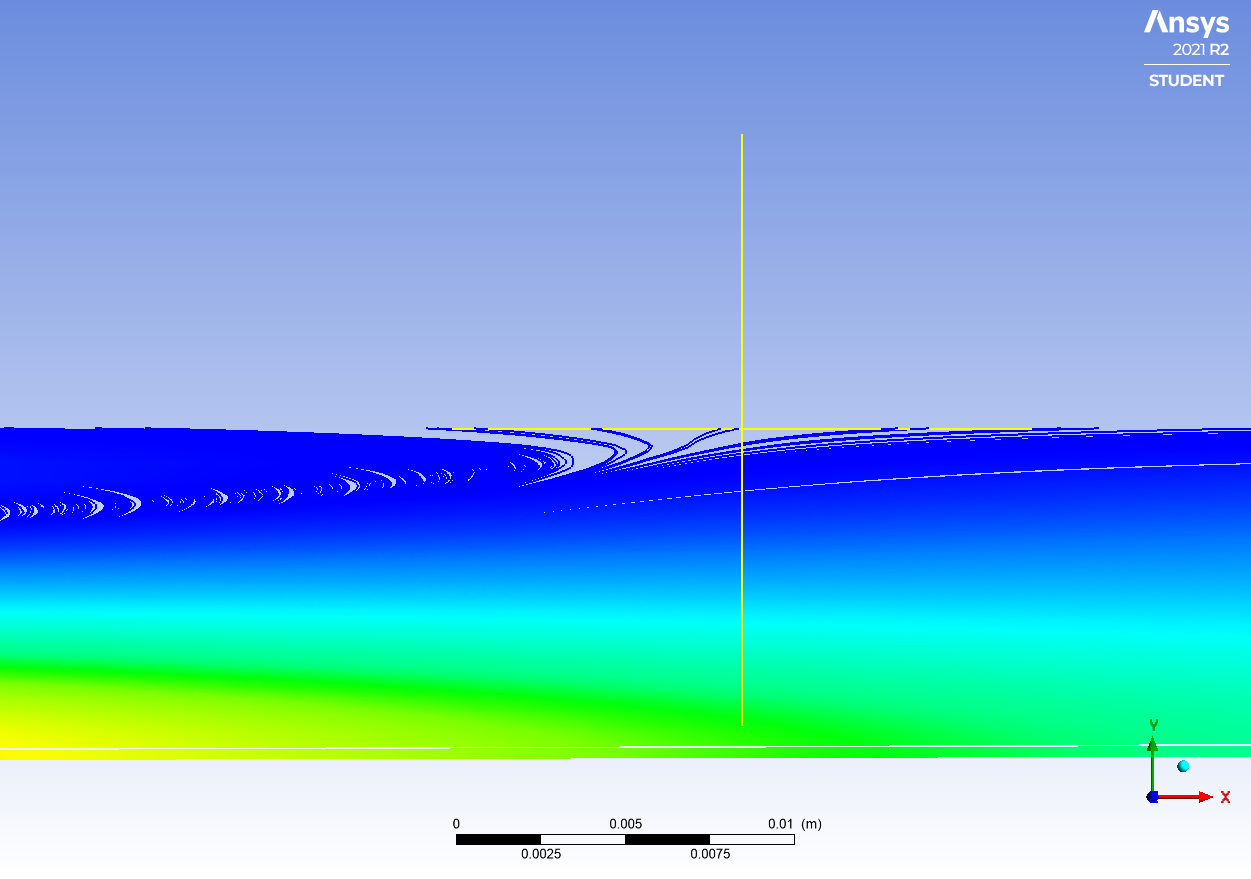
\includegraphics[width=.95\linewidth]{images/task1/100_attachement_0_430.png}
  \subcaption{}
  \label{fig:reat_c}
\end{subfigure}
\hfill
\begin{subfigure}{.75\textwidth}
  \centering
  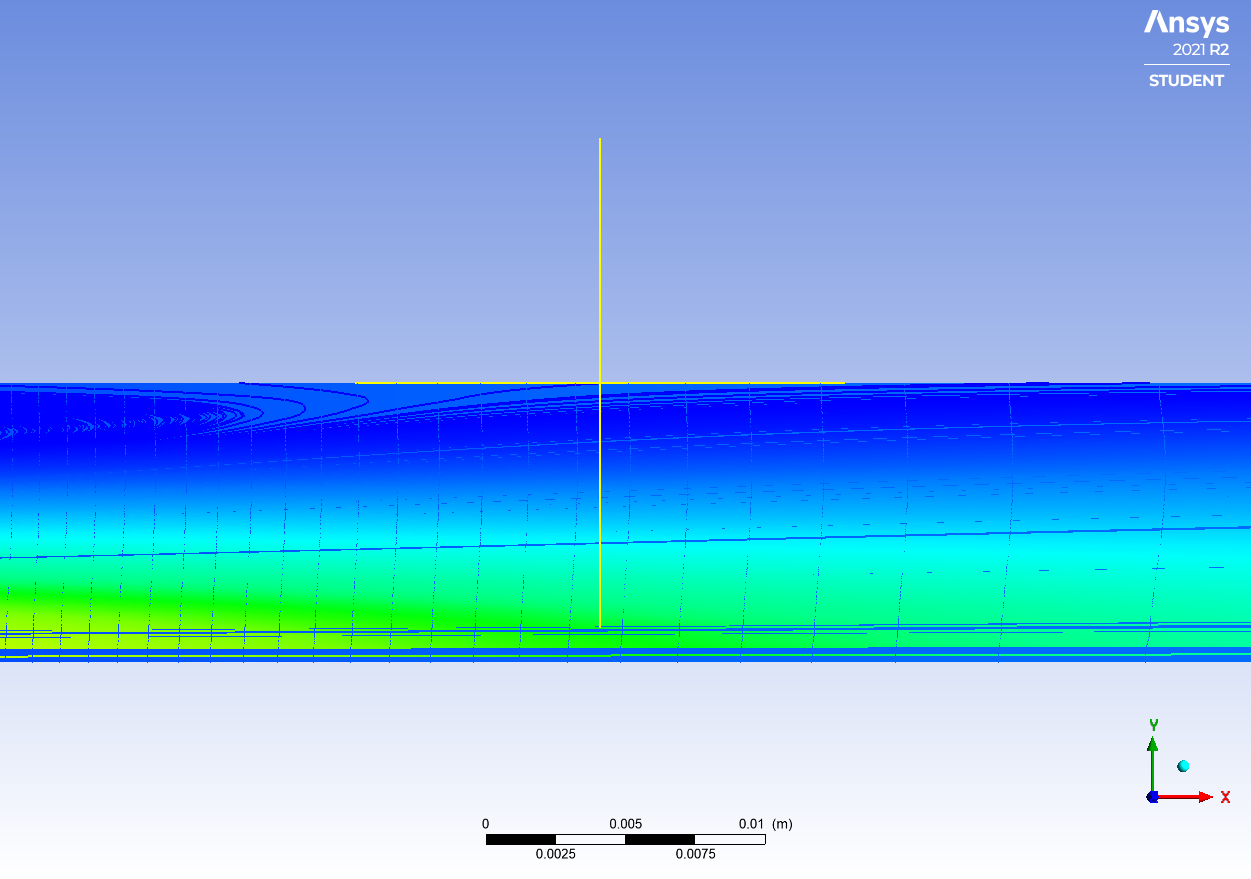
\includegraphics[width=.95\linewidth]{images/task1/150_attachement_0_0681.png}
  \subcaption{}
  \label{fig:reat_d}
\end{subfigure}
\caption{Reattachment Points for 4 different Reynolds numbers.}
\label{fig:reattach}
\end{figure}



